\documentclass[12pt,a4paper]{article}
\usepackage[utf8]{inputenc}
\usepackage[T1]{fontenc}
\usepackage[brazilian]{babel}
\usepackage{color, url}
\usepackage{comment}
\usepackage{graphicx}



\pagestyle{headings}
\markright{}
<<<<<<< HEAD

\topmargin       -1cm

\headheight      1cm
\headsep         1cm

\oddsidemargin -5mm
\evensidemargin  -5mm

\textwidth 16.7cm
\textheight 23.5cm
\baselineskip -13pt



\setlength{\parskip}{0.5cm}
\setlength{\parindent}{1cm}
=======
\topmargin 0cm
\oddsidemargin -0.5mm
\textwidth 16.3cm
\textheight 24cm
%\setlength{\parskip}{0.5cm}
%\setlength{\parindent}{1cm}
>>>>>>> d9c64844eb36beb6480182accad13779f92ccf18



\title{Projeto Final de LPG0002}
\author{Claudio Cesar de Sá e Outros\\ 
	Universidade do Estado de Santa Catarina -- UDESC\\
	Departamento de Ciência da Computação -- DCC\\
	Joinville -- SC\\
	\textcolor{red}{\textbf{Projeto em constante revisão: \today}}
	}


\begin{document}

\maketitle


\tableofcontents


\newpage
\section{Sistema de Índice de Massa Corporal}

A proposta deste sistema é gerenciar Peso $\times $ Altura de toda turma de LPG0002,
bem como dar conselhos se alguém estiver acima ou abaixo do peso. Em resumo,
vamos estender e especificar melhor o exercício passado em sala de aula.



\subsection{Requisitos Técnicos}

\begin{enumerate}
  \item Usar uma estrutura mínima no arquivo de uma estrutura que se segue:
  
\begin{verbatim}
structuc registro_tipo
        {
          char nome[20];
          float altura;
          float  peso;
          char sexo;
        }
\end{verbatim}



\item Podem usar arquivo texto ou binário para este sistema. Cada um tem suas vantagens.

\item Os detalhes técnicos do sistema saúde tem por base o site:
\url{http://www.calculoimc.com.br/tabela-de-imc/}

\end{enumerate}

\subsection{Requisitos Operacionais}

\begin{enumerate}
  \item Um menu principal, com opções, que exiba toda funcionalidade de seu sistema. Deve ser feito em uma função;
  \item Uma opção para cadastrar/incluir pessoas (nome), peso, idade e sexo. Deve ser feito em uma função;
  \item Uma opção para excluir uma pessoa via nome. Deve  ser feito em uma função;

  \item Uma opção para um relatório que exiba o IMC de cada  pessoa via nome e sexo. Deve ser feito em uma função;
  
  \item Uma opção para um relatório que exiba o IMC de cada  pessoa, contudo, com um filtro quanto ao  sexo, deve ser feito em uma função. Exemplo: IMC de todos os homens (h) ou IMC de todas as mulheres (m);
  
  \item Um sistema que forneça aconselhamento as pessoas quanto ao seu IMC
  
   
  \item Uma opção que permita alteração do registro de  uma pessoa, acessando  via nome,
  e alterando TODOS os seus dados. Deve  ser feito em uma função;
  
  
  \item Uma opção para \textit{back-up} do arquivo de dados
  
  \item Uma opção para ler a partir de um arquivo pré-existente, pode ser o restaurar 
   \textit{back-up}
   
   \item .....
   
 \item Na  medida das dúvidas vou respondendo aqui neste item ....
  
\end{enumerate}




\subsection{Procedimento de Entrega}


\begin{enumerate}
  \item Jamais compacte arquivos fontes ... sao muito pequenos ... nao se de este trabalho
  \item Contudo junte-os com o comando \texttt{tar} do linux
    \item \texttt{NENHUM NOME DE ARQUIVOS PODE TER ESPAçOS EM BRANCO}
    \item Em cada arquivo, coloque os nomes
    \item Um arquivo .TXT de como se usa o seu sistema
    \item Após todos arquivos juntos, com nomes sem espaços, o envio será eletrônico
    
\end{enumerate}

\newpage
\section{Sistema de  Entregar}

Como Entregar:
\begin{enumerate}
  \item Acesse: \url{https://dropitto.me/LPG0002_2015_2}
  \item Terá uma senha de acesso comum para turma: \texttt{lpg20152}
    \item Faça \textit{upload} conforme solicitado
    \item Confira o \textit{upload} abaixo na página
    
\end{enumerate}



\subsection{Prazo de Entrega}


\begin{enumerate}
  \item Até o dia 30/novembro -- após as correções solicitadas pelo professor
  \item DEFESAS: dia 30/novembro (dupla presente)
    \item Exame Final: 07/dezembro (favor conferir no Calendário Acadêmico)
    
\end{enumerate}
 
\newpage
\section{Avaliação dos Projetos}

\subsection{Um Guia Global}
Basicamente estarei seguindo a metodologia descrita
em \ref{fig_aval_01}.

 \begin{figure}[!ht]
   \begin{center}
%  \framebox{ 
     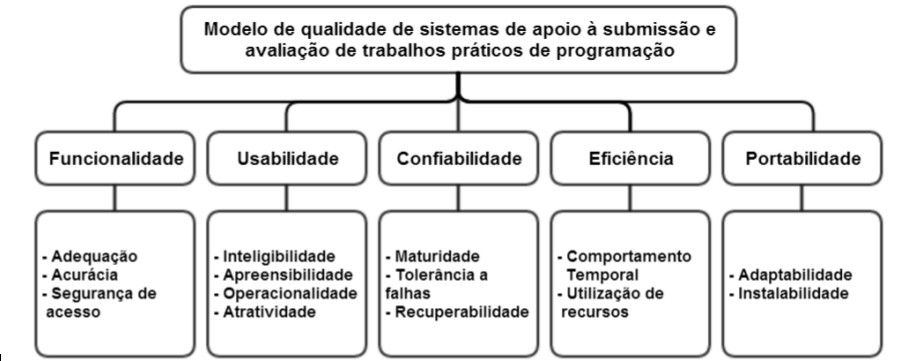
\includegraphics[scale=0.55]{fig_avaliacao_pgms_01.jpg}
%    } 
   
     \caption{Avaliação e Critérios}
       \label{fig_aval_01} %% DEVE VIR depois do CAPTION ... nem eu sabia...
   \end{center}
 \end{figure}



\subsection{Detalhando Alguns Critérios da Avaliação (nota)}


\begin{enumerate}
  \item Funcionando ou não?
  \item Uso de funções. Modularidade.
    \item Uso de ponteiros nas funções.
    \item Adicionais ao que foi solicitado.
    \item Todas opções funcionando.
    \item Uso de qual tipo de arquivo.
     \item A defesa do projeto. As duplas terão que explicar ao professor
     todo sistema, e o mesmo poderá fazer perguntas e solicitações de mudanças.
     \item As mudanças deverão ser feitas no dia 30/novembro mesmo.
     \item \textbf{TODA DEFESA FEITA ANTES DESTA DATA SERA COMPUTADA POSITIVAMENTE NA NOTA}
     \item Cuidar com a usabilidade ... não é interessante ter que digitar \textit{MUIIIIIII.........IIIIIITO}!
     
    
\end{enumerate}


\subsection{Especificando Outros}

A figura \ref{fig_aval_02} deve ser adaptada. Troque a palavra \textbf{Curso} da 
figura \ref{fig_aval_02} por \textbf{registo }ou \textbf{ficha da pessoa}.

 \begin{figure}[!hb]
   \begin{center}
%  \framebox{ 
     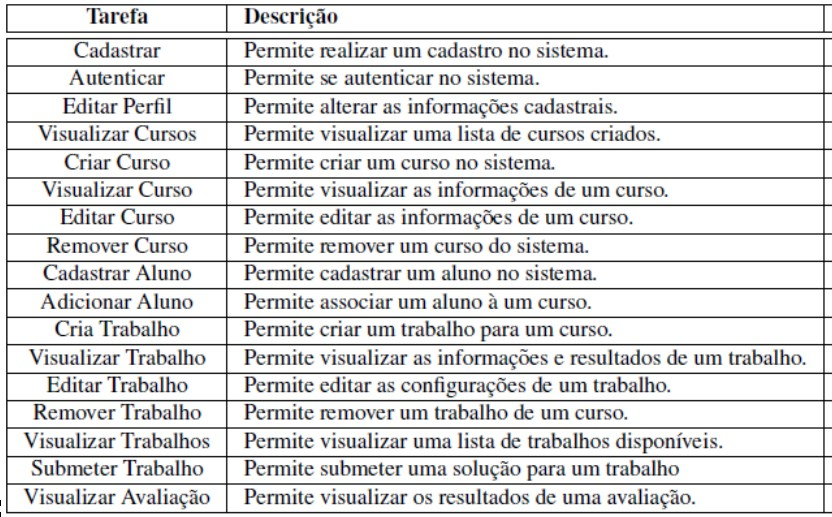
\includegraphics[scale=0.55]{fig_avaliacao_pgms_02.jpg}
%    } 
   
     \caption{Avaliação e Critérios -- ADAPTADOS AO PROJETO DO CURSO}
       \label{fig_aval_02} %% DEVE VIR depois do CAPTION ... nem eu sabia...
   \end{center}
 \end{figure}
 
\end{document}
